%! Author = Swagmaster
%! Date = 11/14/2022

% Preamble
\documentclass[11pt,twocolumn]{article}


% Packages
\usepackage{graphicx}
\usepackage{subcaption}
\title{Report}
\author{Gregor von Laszewski, Jacques Fleischer, Geoffrey C. Fox}

% Document
\begin{document}
\maketitle

\begin{abstract}

My abstract

\end{abstract}

\tableofcontents

\section{Benchmark Terminology}

\begin{tabular}{rl}
NNSE & 2 Week Intervals \\
\hline
Year Back & \\ % describe each one of these values
2wk+7AVG & \\ % what does 2 wk 7 avg mean?
2wk+13AVG & \\
6 Months Back & \\
2wk+13AVG & \\
3 Months Back & \\
2wk+7AVG & \\
2wk+7AVG & \\
2wk+26AVG & \\
2wk+26AVG & \\
2wk+13AVG & \\
2wk+26AVG & \\
2wk+7AVG & \\
2wk+13AVG & \\
2 weeks Now & \\
2wk+26AVG & \\
\hline
\end{tabular}

\section{Results from Rivanna V100}

Rivanna is a supercomputer located at the University
of Virginia. It has a variety of CUDA cards, including
an A100, V100, K80. In this benchmark we use its V100.

\subsection{Best Accuracy}

Just one entry for best accuracy.

\subsection{Accuracy Comparison}

We compare accuracy.

\subsection{Time Comparison}

We compare time.

\subsection{Power Consumption}

We compare power.

Hello. testing~\cite{las21openapi}.

\section{figure}

\begin{figure*}[p]
     \centering
     \begin{subfigure}[b]{0.49\textwidth}
        \centering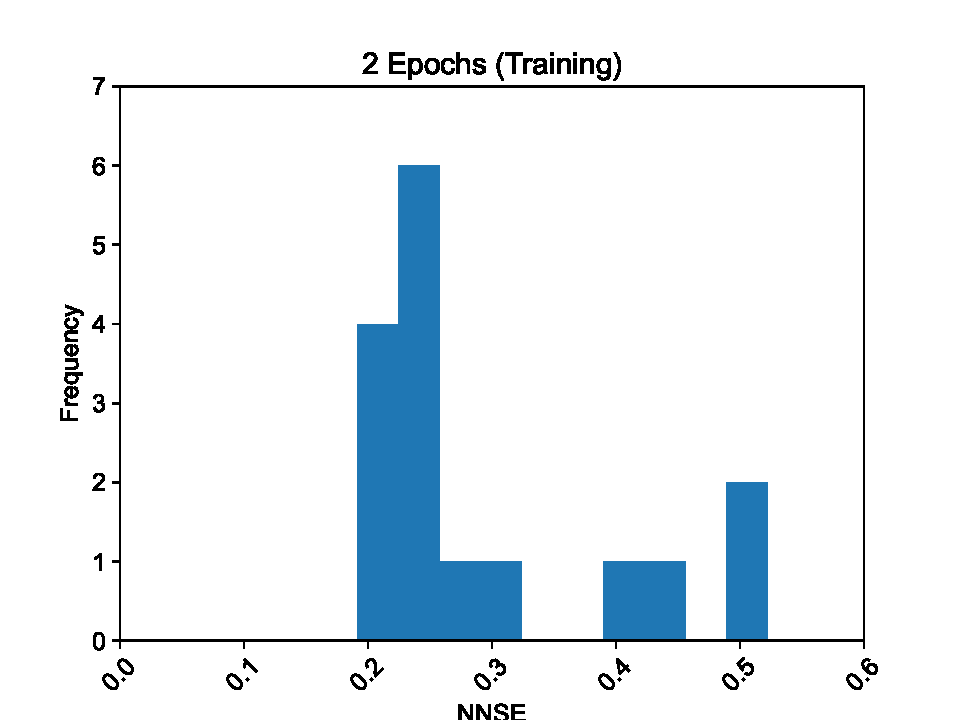
\includegraphics[width=1.0\linewidth]{images/2_training-NNSE.pdf}
        \caption{NNSE - 2 epochs}
        \label{fig:tbd1}
     \end{subfigure}
     \hfill
     \begin{subfigure}[b]{0.49\textwidth}
        \centering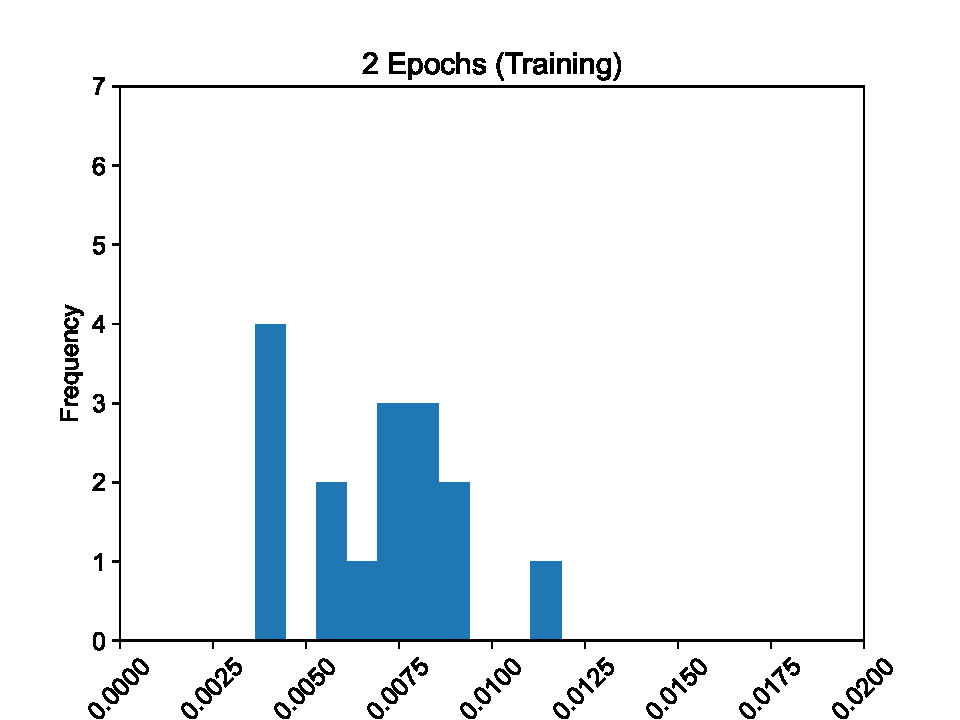
\includegraphics[width=1.0\linewidth]{images/2_training-MSE.pdf}
        \caption{MSE - 2 epochs}
        \label{fig:tbd2}
     \end{subfigure}
     \hfill
     \newline
     \begin{subfigure}[b]{0.49\textwidth}
        \centering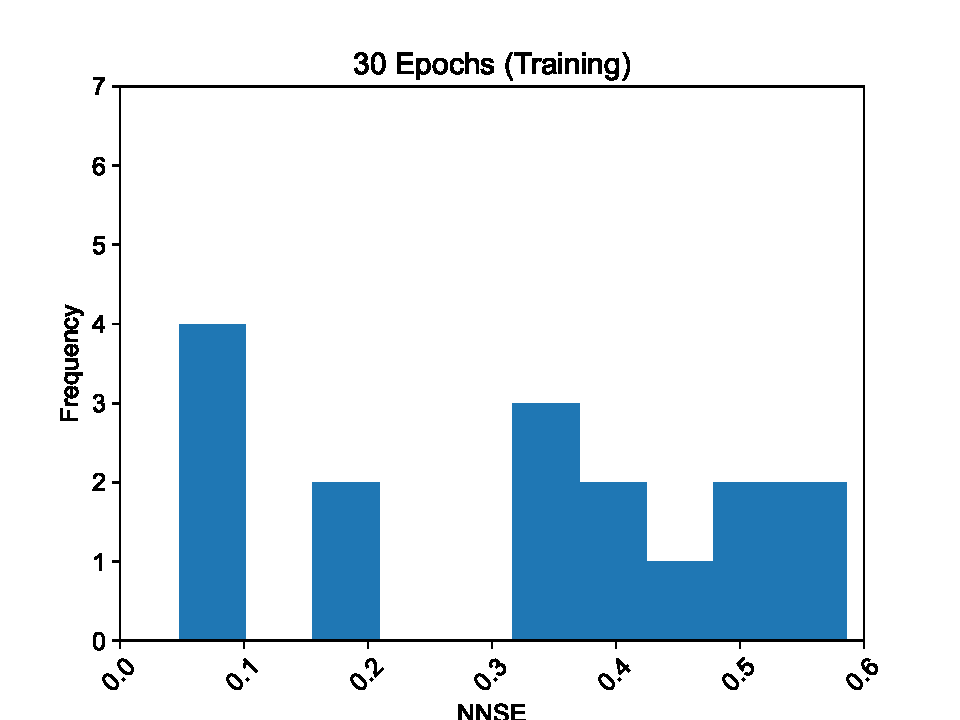
\includegraphics[width=1.0\linewidth]{images/30_training-NNSE.pdf}
        \caption{NNSE - 30 epochs}
        \label{fig:tbd3}
     \end{subfigure}
     \hfill
     \begin{subfigure}[b]{0.49\textwidth}
        \centering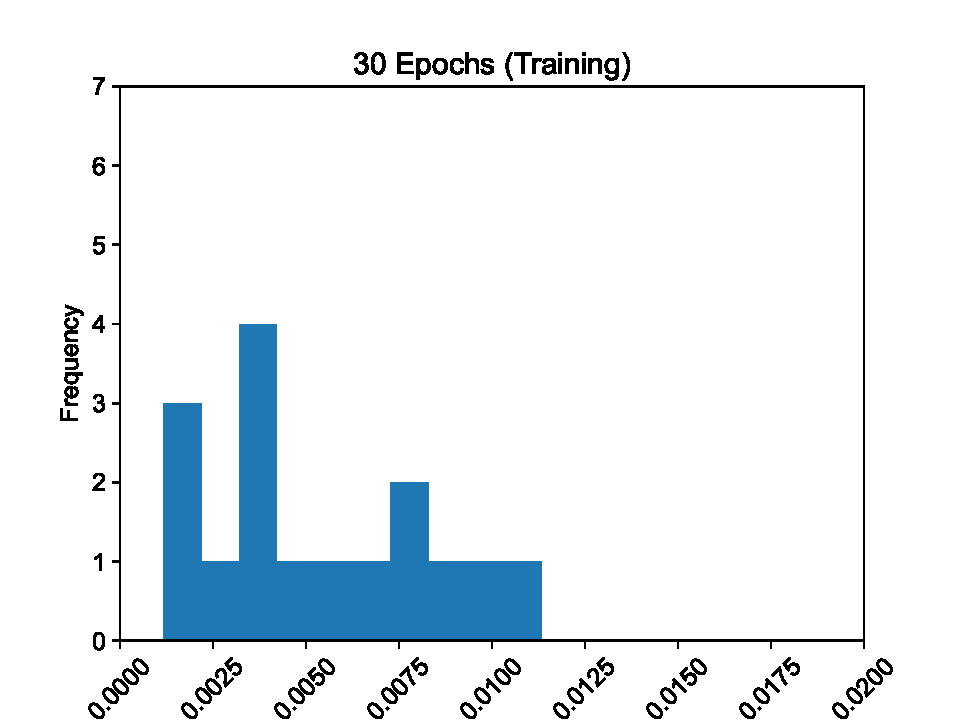
\includegraphics[width=1.0\linewidth]{images/30_training-MSE.pdf}
        \caption{MSE - 30 epochs}
        \label{fig:tbd4}
     \end{subfigure}
     \hfill
          \newline
     \hfill
     \begin{subfigure}[b]{0.49\textwidth}
        \centering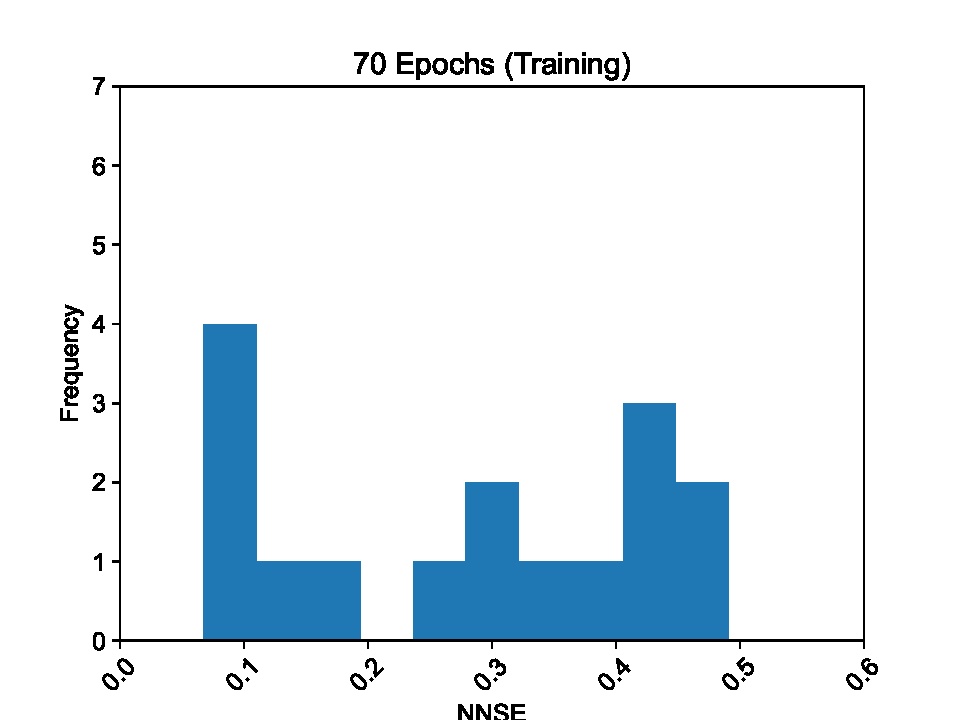
\includegraphics[width=1.0\linewidth]{images/70_training-NNSE.pdf}
        \caption{NNSE - 70 epochs}
        \label{fig:tbd3}
     \end{subfigure}
     \hfill
     \begin{subfigure}[b]{0.49\textwidth}
        \centering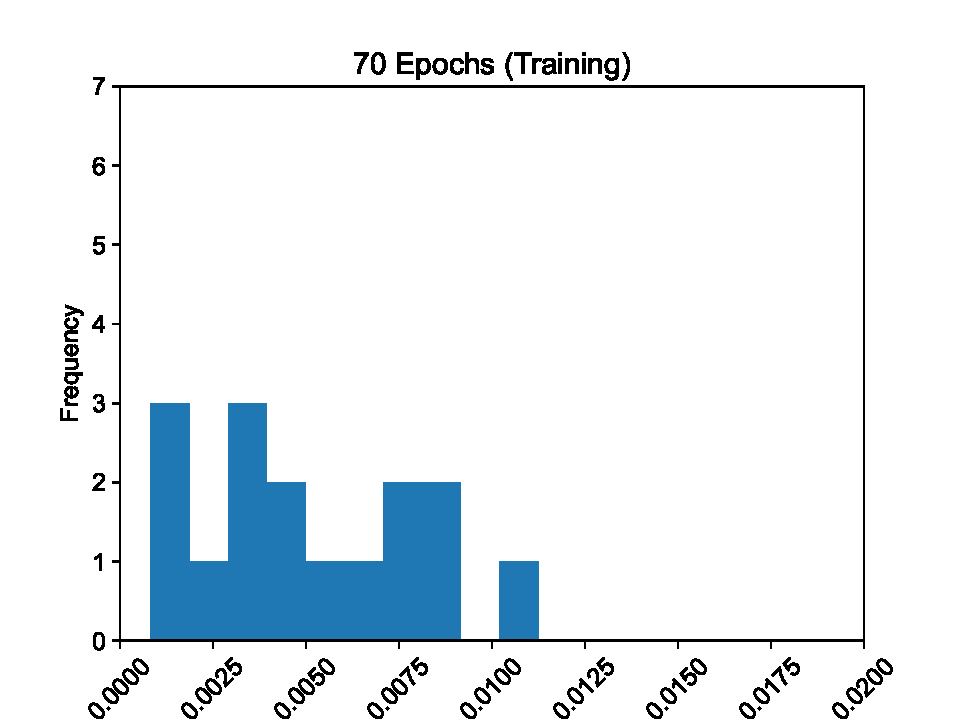
\includegraphics[width=1.0\linewidth]{images/70_training-MSE.pdf}
        \caption{MSE - 70 epochs}
        \label{fig:tbd4}
     \end{subfigure}
        \caption{NNSE and MSE values for epochs 2, 30, 70 (training).}
        \label{fig:six graphs}
\end{figure*}

\begin{figure}[htb]
%\centering\includegraphics[width=1.0\columnwidth]{usecase/images/hvac-new-arch.png}
\centering\includegraphics[width=1.0\columnwidth]{images/2-weeks-now.pdf}
\caption{To be determined}
\label{fig:tbd}
\end{figure}

\begin{table}[htb]
%\centering\includegraphics[width=1.0\columnwidth]{usecase/images/hvac-new-arch.png}

\caption{To be determined}
\label{tab:tbd}
\bigskip
%\resizebox{1.0\columnwidth}{!}{%
\centering\begin{tabular}{rl}
NNSE & name \\
\hline
0.191300 & Year Back \\
0.192700 & 6M 2wk+7AVG \\
0.197000 & 6M 2wk+13AVG \\
0.201600 & 6 Months Back \\
0.232600 & 1Y 2wk+13AVG \\
0.233000 & 3 Months Back \\
0.235800 & 1Y 2wk+7AVG \\
0.243000 & 3M 2wk+7AVG \\
0.251600 & 1Y 2wk+26AVG \\
0.251700 & 6M 2wk+26AVG \\
0.278800 & 3M 2wk+13AVG \\
0.302500 & 3M 2wk+26AVG \\
0.405600 & Now 2wk+7AVG \\
0.429900 & Now 2wk+13AVG \\
0.506800 & 2 weeks Now \\
0.521800 & Now 2wk+26AVG \\
\hline
\end{tabular}%
%}
\end{table}

\begin{table}[htb]
%\centering\includegraphics[width=1.0\columnwidth]{usecase/images/hvac-new-arch.png}

\caption{To be determined}
\label{tab:tbdetermined}
\bigskip
%\resizebox{1.0\columnwidth}{!}{%
\centering\begin{tabular}{rl}
NNSE & 2 Week Intervals \\
\hline
0.195200 & 6M 2wk+7AVG \\
0.201000 & 6 Months Back \\
0.201600 & 6M 2wk+13AVG \\
0.204500 & Year Back \\
0.219700 & 3 Months Back \\
0.228900 & 3M 2wk+7AVG \\
0.238200 & 1Y 2wk+13AVG \\
0.249500 & 1Y 2wk+7AVG \\
0.264400 & 6M 2wk+26AVG \\
0.266200 & 3M 2wk+13AVG \\
0.270300 & 1Y 2wk+26AVG \\
0.295800 & 3M 2wk+26AVG \\
0.379700 & Now 2wk+7AVG \\
0.412700 & Now 2wk+13AVG \\
0.470100 & 2 weeks Now \\
0.502300 & Now 2wk+26AVG \\
\hline
\end{tabular}%
%}
\end{table}

\section*{Acknowledgements}

Continued work was in part funded by the NSF CyberTrain-
ing: CIC: CyberTraining for Students and Technologies from
Generation Z with the award numbers 1829704 and 2200409
and NIST 60NANB21D151T.


\bibliographystyle{IEEEtran}
\bibliography{report.bib}

\end{document}